\documentclass[11pt,a4paper]{article}

\usepackage[margin=2.5cm]{geometry}
\usepackage{amsmath, amssymb, amsthm}
\usepackage{listings}
\usepackage{xcolor}
\usepackage{hyperref}
\usepackage{enumitem}
\usepackage{booktabs}
\usepackage{tikz}
\usetikzlibrary{positioning, arrows.meta, shapes.geometric}
\usepackage{titlesec}
\usepackage{parskip}

\hypersetup{
    colorlinks=true,
    linkcolor=blue!50!black,
    urlcolor=blue!50!black,
    citecolor=blue!50!black,
}

\definecolor{codebg}{rgb}{0.97,0.97,0.97}
\definecolor{codekw}{rgb}{0.0,0.2,0.6}
\definecolor{codestr}{rgb}{0.6,0.1,0.1}
\definecolor{codecomment}{rgb}{0.4,0.4,0.4}

\lstdefinestyle{py}{
    language=Python,
    backgroundcolor=\color{codebg},
    basicstyle=\ttfamily\small,
    keywordstyle=\color{codekw}\bfseries,
    stringstyle=\color{codestr},
    commentstyle=\color{codecomment}\itshape,
    frame=single,
    framesep=4pt,
    framerule=0pt,
    rulecolor=\color{codebg},
    breaklines=true,
    showstringspaces=false,
    columns=fullflexible,
    xleftmargin=8pt,
    xrightmargin=8pt,
}
\lstset{style=py}

\titleformat{\section}{\large\bfseries}{\thesection}{0.6em}{}
\titleformat{\subsection}{\normalsize\bfseries}{\thesubsection}{0.6em}{}

\newcommand{\code}[1]{\texttt{\small #1}}
\newcommand{\file}[1]{\texttt{\small #1}}
\newcommand{\R}{\mathbb{R}}
\newcommand{\Rmat}[1]{R(#1)}

\title{\texttt{sim2d} / mobilebarrier --- Integration Plan}
\author{Project: autonomous robotic motorway barriers}
\date{Current as of refactor: architecture skeleton complete}

\begin{document}
\maketitle

\begin{abstract}
\noindent
This document is a step-by-step integration plan for filling out the
\code{sim2d} library and the \code{mobilebarrier} project on top of the
architecture skeleton already in place. It is intended to be worked through
sequentially: each phase has a stated goal, the dependencies it relies on,
the maths needed, implementation sketches, validation steps, and common
pitfalls. A reader who follows it end-to-end should arrive at a working 2D
simulation capable of testing navigation and signal-conditioning algorithms
for the motorway barrier robot, with a clean library underneath that the
wider university group can reuse.
\end{abstract}

\tableofcontents
\vspace{1em}\hrule\vspace{1em}

% ============================================================================
\section{How to use this document}

The plan is organised as a sequence of phases. \textbf{Do not work on phases
out of order} unless you understand the dependency graph well enough to
justify it --- almost every later phase assumes the body dynamics
(Phase~\ref{sec:body}) and plant integration (Phase~\ref{sec:plant}) are
done. Each phase contains:

\begin{description}[leftmargin=1.5em, style=nextline]
    \item[Goal.] What "done" looks like, expressed as a behaviour you can
        observe.
    \item[Depends on.] Earlier phases (or external bits of code) that must
        be in place first.
    \item[Maths.] The equations you'll need to implement. Brief; full
        derivations are in the appendix.
    \item[Implementation tasks.] A checklist with rough function
        signatures.
    \item[Validation.] How to verify the phase is correct in isolation,
        before wiring it into the full loop.
    \item[Pitfalls.] Bugs the design naturally invites; flag them early.
\end{description}

\textbf{Working style suggestion:} resist the urge to perfect any single
phase. The goal is end-to-end closure first (Phases~\ref{sec:body}--%
\ref{sec:control}, with cheap stubs for sensors and estimation), then
fidelity. A working closed loop with crap stubs everywhere is more useful
than a perfect EKF that has nothing to filter.

% ============================================================================
\section{Architecture recap}

\begin{center}
\begin{tikzpicture}[
    node distance=0.6cm and 1.2cm,
    box/.style={rectangle, draw, rounded corners, minimum height=0.9cm, minimum width=2.4cm, align=center, font=\small},
    bigbox/.style={rectangle, draw, dashed, rounded corners, inner sep=0.4cm},
    arrow/.style={-{Stealth}, thick},
]
    \node[box] (body) {Body \\ (\code{RigidBody2D})};
    \node[box, right=of body] (hg) {HardwareGroup \\ (drivetrain)};
    \node[box, right=of hg] (sensors) {Sensors \\ (extra)};

    \node[box, below=1.4cm of body] (estimator) {StateEstimator};
    \node[box, right=of estimator] (supervisor) {Supervisor};
    \node[box, right=of supervisor] (behaviours) {Behaviours \\ (Cruise, Dock)};

    \begin{scope}[on background layer]
        \node[bigbox, fit=(body)(hg)(sensors), label=above:\textbf{Plant (truth-side)}] (plant) {};
        \node[bigbox, fit=(estimator)(supervisor)(behaviours), label=below:\textbf{Stack (onboard-side)}] (stack) {};
    \end{scope}

    \draw[arrow] (sensors.south) -- ++(0,-0.3) -| (estimator.north) node[midway, above, font=\scriptsize] {measurements};
    \draw[arrow] (hg.south) -- ++(0,-0.3) -| (estimator.north) node[pos=0.25, above, font=\scriptsize] {};
    \draw[arrow] (estimator.east) -- (supervisor.west) node[midway, above, font=\scriptsize] {state};
    \draw[arrow] (supervisor.east) -- (behaviours.west) node[midway, above, font=\scriptsize] {active};
    \draw[arrow] (behaviours.north) -- ++(0,0.3) -| (hg.south) node[pos=0.75, right, font=\scriptsize] {commands};
\end{tikzpicture}
\end{center}

The Plant is the truth side of a robot --- physical body, motors, sensors.
The Stack is the autonomy side --- the same code that would run on real
hardware. The boundary between them is the most architecturally important
seam in the codebase.

\code{World.step(dt)} is strictly two-phase:
\begin{enumerate}
    \item For every robot, read sensors that are due, run the estimator,
        let the supervisor pick a behaviour, compute a command, and stage
        it on the actuators. \emph{Read-only on plant state.}
    \item Integrate every plant and every world body forward by \code{dt}.
        \emph{Write phase.}
\end{enumerate}
This guarantees no robot ever sees a partially-updated world during its
decide phase.

% ============================================================================
\section{Conventions}

\subsection{Frames}

\begin{description}[leftmargin=1.5em, style=nextline]
    \item[World frame $W$.] Right-handed 2D Cartesian. $+x$ east, $+y$
        north, $+\theta$ counter-clockwise.
    \item[Body frame $B$.] Origin at the body's centre of mass, $+x$
        forward, $+y$ left, $+\theta$ counter-clockwise (rotation about $z$
        out of plane). Aligned with $W$ when $\theta = 0$.
\end{description}

The rotation from body to world is
\begin{equation}
    \Rmat{\theta} =
    \begin{bmatrix} \cos\theta & -\sin\theta \\ \sin\theta & \cos\theta \end{bmatrix}.
    \label{eq:rot}
\end{equation}
A vector $v_B$ in the body frame is expressed in the world frame as
$v_W = \Rmat{\theta}\, v_B$.

\subsection{State variables}

For a planar rigid body:
\begin{align}
    q     &= [x,\ y,\ \theta]^\top      &\text{(pose, world frame)} \\
    v     &= [v_x,\ v_y,\ \omega]^\top  &\text{(velocity, world frame)} \\
    F     &= [F_x,\ F_y,\ \tau_z]^\top  &\text{(wrench, world frame)}
\end{align}
The accumulated wrench is cleared on each integrate call. Linear and
angular components are kept in the same vector for ergonomics --- the only
place this matters is in the mass matrix
$M = \mathrm{diag}(m, m, I_{zz})$ used in the equations of motion.

\subsection{Code style and naming}

Module names are \code{snake\_case}, classes are \code{PascalCase}, all
imports are absolute (\code{from sim2d.core.plant import Plant}). Type
hints everywhere; \code{from \_\_future\_\_ import annotations} at the top
of every file that has forward references. Library code (\code{sim2d/}) must
not import from \code{mobilebarrier/} --- enforce with a quick grep in CI
once tests are set up.

% ============================================================================
\section{Phase 1 --- Body dynamics}
\label{sec:body}

\subsection*{Goal}
A free \code{RigidBody2D} with mass $m$ and inertia $I_{zz}$, when given a
constant wrench, accelerates correctly; when free of wrench, drifts at
constant velocity; integrates pose forward via Euler.

\subsection*{Depends on}
\code{InertiaMatrix} and the inertia primitives (already in place).

\subsection*{Maths}

Equations of motion:
\begin{equation}
    M\dot{v} = F, \qquad
    M = \begin{bmatrix} m & 0 & 0 \\ 0 & m & 0 \\ 0 & 0 & I_{zz} \end{bmatrix}.
    \label{eq:eom}
\end{equation}
Component-wise: $\dot{v}_x = F_x/m$, $\dot{v}_y = F_y/m$, $\dot{\omega} = \tau_z/I_{zz}$.

Two integration schemes worth knowing:
\begin{description}
    \item[Explicit Euler.] $v_{k+1} = v_k + \dot{v}\, \Delta t$;\quad $q_{k+1} = q_k + v_k\, \Delta t$.
        Simple. Energy-positive on rotational motion --- a frictionless spinner will accelerate
        spuriously over long runs.
    \item[Semi-implicit (symplectic) Euler.] $v_{k+1} = v_k + \dot{v}\, \Delta t$;\quad
        $q_{k+1} = q_k + v_{k+1}\, \Delta t$. Same code complexity, much
        better long-term energy behaviour. \textbf{Recommended default.}
\end{description}
Heading wrap: after each step, fold $\theta$ back into $(-\pi, \pi]$ via
$\theta \leftarrow ((\theta + \pi) \bmod 2\pi) - \pi$. Otherwise $\theta$
grows unboundedly and any modulo-sensitive controller will blow up at
$\pm \pi$.

\subsection*{Implementation tasks}

In \file{sim2d/bodies/rigid\_body\_2d.py}:

\begin{lstlisting}
class RigidBody2D(Body):
    def __init__(self,
            mass: float,
            inertia: InertiaMatrix,
            init_pose: np.ndarray | None = None):
        # store mass, inertia
        # init pose to zeros(3) or copy of init_pose
        # init velocity zeros(3)
        # init wrench accumulator zeros(3)

    def apply_wrench(self, wrench: np.ndarray) -> None:
        # accumulate; do NOT integrate here

    def integrate(self, dt: float) -> None:
        # acceleration from wrench / mass + inertia
        # semi-implicit Euler: update velocity then pose
        # wrap heading
        # zero wrench accumulator
\end{lstlisting}

In \file{sim2d/bodies/body.py}: change the abstract method to
\code{integrate(self, dt: float) -> None} so the world can pass \code{dt}
to both robots and bodies uniformly.

In \file{sim2d/core/world.py}: in Phase 2 of \code{step()}, replace
\code{body.update()} with \code{body.integrate(dt)}.

\subsection*{Validation}

Write \file{tests/test\_rigid\_body\_2d.py}:
\begin{itemize}
    \item \textbf{Drift test.} No wrench, initial velocity $(1, 0, 0)$.
        After $t = 5\,\text{s}$, pose should be $(5, 0, 0)$ to within
        floating-point error.
    \item \textbf{Constant force test.} $F_x = m$ (so expected
        $a = 1\,\text{m/s}^2$). After $t = 1\,\text{s}$ from rest, velocity
        should be $\approx 1\,\text{m/s}$, pose $\approx 0.5\,\text{m}$.
    \item \textbf{Constant torque test.} Pure $\tau_z$, check
        $\omega \to \tau/I_{zz}$.
    \item \textbf{Heading wrap.} Apply enough $\tau$ for many revolutions;
        check $\theta$ stays in $(-\pi, \pi]$.
\end{itemize}

\subsection*{Pitfalls}

\begin{itemize}
    \item Forgetting to clear the wrench accumulator. Forces will silently
        compound across ticks.
    \item Using explicit Euler and then puzzling over slow energy growth
        in a frictionless test.
    \item Storing velocity in the body frame rather than the world frame.
        Pick one and document it; mixing them is an infinite source of
        sign errors. The plan recommends world frame for storage.
\end{itemize}

% ============================================================================
\section{Phase 2 --- Plant integration}
\label{sec:plant}

\subsection*{Goal}
Given staged commands on a drivetrain's actuators, the plant's body moves
correctly. Validated open-loop: a constant wheel-velocity command produces
the expected mecanum trajectory (e.g.\ pure forward, pure strafe, pure
rotation, diagonal).

\subsection*{Depends on}
Phase~\ref{sec:body}; mecanum kinematics (already in place); ideal actuator
(Phase~\ref{sec:actuators}, but you can stub it inline first).

\subsection*{Two integration modes}

You have a choice for \code{Plant.integrate(dt)}:

\paragraph{Kinematic mode (recommended for first close-of-loop).}
Treat wheel velocities as ground-truth: read commanded $\dot\theta_i$ from
the actuators, run forward kinematics to get body-frame velocity
$v_B = K^+ (\dot\theta\, r)$, rotate to world frame and write directly into
\code{body.velocity}. Then \code{body.integrate(dt)} steps pose. No forces,
no slip, no inertia. Inertia is irrelevant in this mode --- which is fine
for nav-algorithm testing where you just want predictable motion.

\paragraph{Dynamic mode (force-based).}
Each wheel applies a tangential force $f_i$ to the chassis. Sum forces and
moment arms to get a body-frame wrench, rotate to world, call
\code{body.apply\_wrench(F\_W)}, then \code{body.integrate(dt)}. This is
where mass and inertia start mattering. The tricky part is the wheel-force
model:
\begin{itemize}
    \item Idealised: $f_i$ is whatever is needed to track the commanded
        wheel speed. Not physical but clean --- equivalent to perfect
        traction.
    \item Realistic: a friction-cone / slip model, where wheel velocity
        differs from contact-point velocity and tangential force is a
        function of slip. Out of scope until later.
\end{itemize}

\textbf{Recommendation:} build kinematic mode first, get the loop closed
end-to-end, then graduate to dynamic mode in a separate phase once you
need it (e.g.\ when motor saturation or wheel slip becomes a research
question).

\subsection*{Maths --- mecanum forward kinematics}

Given the inverse kinematics already implemented,
\begin{equation}
    \dot\theta_i \cdot r = J_i \cdot v_B,\qquad
    J_i = [1,\ s_i,\ s_i p_x^i - p_y^i],
\end{equation}
where $s_i \in \{-1, +1\}$ depending on roller orientation per wheel
(see \code{MecanumKinematics.\_S}), $r$ is wheel radius, $(p_x^i, p_y^i)$
is wheel position in body frame.

For four wheels we get an over-determined system $J\, v_B = r\, \dot\theta$
which is solved by the Moore--Penrose pseudo-inverse already used in
\code{FK}. World-frame velocity is then
\begin{equation}
    v_W = \begin{bmatrix} \Rmat{\theta} & 0 \\ 0 & 1 \end{bmatrix} v_B.
    \label{eq:body2world}
\end{equation}

\subsection*{Implementation tasks}

In \file{sim2d/core/plant.py}, fill out \code{integrate(dt)}:

\begin{lstlisting}
def integrate(self, dt: float) -> None:
    # Kinematic mode for now
    for hg in self.hardware_groups:
        hg.integrate(dt)  # advances actuator dynamics
        if hg.kinematics is not None:
            wheel_speeds = np.array([a.velocity for a in hg.actuators])
            v_body = hg.kinematics.FK(wheel_speeds)
            R = rotation_matrix_2d(self.body.pose[2])
            v_world = np.zeros(3)
            v_world[:2] = R @ v_body[:2]
            v_world[2] = v_body[2]
            self.body.velocity = v_world
    self.body.integrate(dt)
\end{lstlisting}

\code{rotation\_matrix\_2d} can live in a utility module, e.g.
\file{sim2d/core/transforms.py}. Don't sprinkle inline rotations through
the codebase --- that is how sign errors hide.

\subsection*{Validation}

Open-loop scenarios in \file{mobilebarrier/scenarios/}:
\begin{enumerate}
    \item \textbf{Forward.} All four wheels at the same speed (with
        appropriate $s_i$ signs). Robot drives along $+x_B$ at the expected
        speed.
    \item \textbf{Strafe.} Diagonally-opposed wheels. Robot drives along
        $+y_B$ without rotating.
    \item \textbf{Spin in place.} Opposite signs across diagonals. Robot
        rotates without translating.
    \item \textbf{Diagonal.} Mix forward and strafe. Should produce a
        $45^{\circ}$ trajectory.
\end{enumerate}
Plot each scenario and eyeball the trajectory before wiring sensors.

\subsection*{Pitfalls}

\begin{itemize}
    \item Forgetting to rotate body-frame velocity into world frame before
        writing to \code{body.velocity}. The robot will drive in the wrong
        direction once it's rotated more than a few degrees.
    \item Mixing up the mecanum sign convention. \code{MecanumKinematics.\_S}
        is order-dependent: changing wheel ordering silently breaks IK/FK.
        Document the wheel order (FL, FR, RL, RR) in a comment near the
        actuator list.
\end{itemize}

% ============================================================================
\section{Phase 3 --- Actuators}
\label{sec:actuators}

\subsection*{Goal}
At minimum, an \code{IdealWheelActuator} that reports back exactly the
commanded velocity. Extension: a first-order DC motor model with
saturation and time constant.

\subsection*{Depends on}
Phase~\ref{sec:body}, Phase~\ref{sec:plant} (the actuator is consumed by
\code{HardwareGroup.integrate}).

\subsection*{Ideal actuator}

\begin{lstlisting}
class IdealWheelActuator(Actuator):
    def __init__(self):
        self.velocity = 0.0
        self._cmd = 0.0
    def command(self, u: np.ndarray) -> None:
        self._cmd = float(u[0])
    def integrate(self, dt: float) -> None:
        self.velocity = self._cmd
\end{lstlisting}

\subsection*{First-order DC motor model (later)}

A linear DC motor with first-order rotor dynamics:
\begin{equation}
    \tau\, \dot\omega + \omega = K_v\, u, \qquad |\omega| \le \omega_{\max}.
\end{equation}
Discretise with $\omega_{k+1} = \omega_k + \frac{\Delta t}{\tau}(K_v u - \omega_k)$
and saturate. Add Coulomb friction or stall torque later if needed. Keep
parameters in a \code{MotorParams} dataclass; pass at construction.

\subsection*{Validation}

\begin{itemize}
    \item \textbf{Step response (DC motor).} Command $u = u_0$ from
        rest; verify exponential rise toward $K_v u_0$ with time constant
        $\tau$.
    \item \textbf{Saturation.} Command beyond $\omega_{\max}$; verify
        velocity clips.
    \item \textbf{Two-phase contract.} \code{command()} alone, with no
        \code{integrate()} call, must not change \code{velocity}. This is
        what enforces the simultaneity invariant in \code{World.step}.
\end{itemize}

% ============================================================================
\section{Phase 4 --- Sensors}
\label{sec:sensors}

\subsection*{Goal}
The plant produces noisy, scheduled measurements that the stack can
consume. At minimum: a \code{PerfectPoseSensor} for debugging.
Production-grade: encoders, IMU (gyro + accel), and a fiducial / dock
marker.

\subsection*{Depends on}
Phase~\ref{sec:body} (sensors read from \code{body.pose} and
\code{body.velocity}); the existing \code{Sensor} ABC and \code{Measurement}
class.

\subsection*{Sensor scheduling}

Each sensor has \code{params.refresh\_rate}. The world calls
\code{sensor.due(t)} during Phase~1 of \code{step()} and only invokes the
sensor if it's due. Update \code{last\_read\_time} after a successful read.

\subsection*{Concrete sensors}

\paragraph{PerfectPoseSensor.} Returns \code{body.pose} unmodified. Use as a
ground-truth reference in tests of the controller and in early sanity
checks of the estimator.

\paragraph{WheelEncoder.} Reads cumulative wheel rotation $\theta_i$ (or
incremental $\Delta \theta_i$ since the last sample). Add quantisation:
\begin{equation}
    \tilde\theta_i = \mathrm{round}(\theta_i / \delta) \cdot \delta,
\end{equation}
where $\delta = 2\pi / N_{\text{ticks}}$. Optionally add Gaussian
quantisation jitter. Encoders feed the dead-reckoner / EKF.

\paragraph{Gyro.} Reads $\omega + b_g + n_g$ where $b_g$ is a slowly drifting
bias (Ornstein--Uhlenbeck or simple random walk) and $n_g \sim
\mathcal{N}(0, \sigma_g^2)$. Bias is the realistic part --- a perfect-noise
gyro is too easy.

\paragraph{Accelerometer.} For 2D, reads body-frame linear acceleration
plus bias and noise. Subtract the centripetal term if the EKF expects
proper acceleration. Skip until you actually need it for fusion.

\paragraph{Fiducial / dock marker.} Returns a relative pose
$(\Delta x_B, \Delta y_B, \Delta \theta_B)$ from robot to a known fiducial,
visible only when the fiducial is within range/angle of the camera. Models
two key failure modes:
\begin{itemize}
    \item \textbf{Dropouts.} Probability of "no detection" rising near the
        FOV edge.
    \item \textbf{Occasional outliers.} A small chance of a wildly wrong
        reading (mis-association). The estimator must handle these
        gracefully --- a chi-square gate on Mahalanobis distance is
        standard.
\end{itemize}

\subsection*{Noise model abstraction}

The existing \code{NoiseModel} ABC is the right shape. Implementations:
\code{GaussianNoise(sigma)}, \code{BiasedGaussianNoise(sigma, bias\_walk)},
\code{LatencyNoise(buffer\_depth)} --- the last one delays a measurement
by a fixed number of ticks, which is critical to test honestly because
real sensors are never instantaneous.

\subsection*{Validation}

\begin{itemize}
    \item Sample a noisy sensor for many ticks, check empirical mean and
        variance against the configured model.
    \item Configure refresh rates of $10\,\text{Hz}$ and $100\,\text{Hz}$
        in the same scenario; verify each fires the right number of times.
    \item Latency: compare delayed measurement against the body's pose
        history at $t - \Delta t$.
\end{itemize}

% ============================================================================
\section{Phase 5 --- State estimation}
\label{sec:estimator}

\subsection*{Goal}
A \code{StateEstimator} that produces a usable belief about the robot's
pose and velocity. Three implementations of increasing fidelity:
\code{PassthroughEstimator}, \code{DeadReckoner}, \code{EKF}.

\subsection*{Depends on}
Phase~\ref{sec:sensors}; the existing \code{StateEstimator} ABC and
\code{MeasurementModel} stub.

\subsection*{Passthrough}

\begin{lstlisting}
class PassthroughEstimator(StateEstimator):
    def __init__(self, perfect_pose_sensor: Sensor):
        self.state = np.zeros(6)
        self.sensor = perfect_pose_sensor
    def predict(self, dt): pass
    def update(self, m: Measurement):
        self.state[:3] = m.z  # x, y, theta straight in
\end{lstlisting}

Useful as a debug stub to factor estimation out of the loop while you
verify the controller and behaviours work.

\subsection*{Dead reckoning from encoders}

\begin{equation}
    v_B = K^+ (\dot\theta\, r), \qquad
    q_{k+1} = q_k + R(\theta_k) v_B\, \Delta t.
\end{equation}
Drifts unboundedly without external aiding --- exactly the role of the
EKF's correction step.

\subsection*{Extended Kalman Filter}

State: $x = [x, y, \theta, v_x, v_y, \omega]^\top \in \R^6$ (world frame).

Process model with control input $u_k$ (commanded body-frame velocity from
the previous tick):
\begin{equation}
    f(x_k, u_k) = x_k +
    \begin{bmatrix} R(\theta_k) u_k^{(xy)} \\ u_k^{(\omega)} \\ 0 \\ 0 \\ 0 \end{bmatrix} \Delta t,
\end{equation}
or, if you prefer to model velocity as part of the state, propagate $q$
with $v$ and $v$ with whatever motion model fits the actuators.

Predict:
\begin{align}
    \hat{x}_{k|k-1} &= f(\hat{x}_{k-1|k-1}, u_k) \\
    P_{k|k-1}       &= F_k P_{k-1|k-1} F_k^\top + Q_k.
\end{align}

Update with measurement $z_k$ and model $h$:
\begin{align}
    y_k       &= z_k - h(\hat{x}_{k|k-1}) \\
    S_k       &= H_k P_{k|k-1} H_k^\top + R_k \\
    K_k       &= P_{k|k-1} H_k^\top S_k^{-1} \\
    \hat{x}_{k|k} &= \hat{x}_{k|k-1} + K_k y_k \\
    P_{k|k}   &= (I - K_k H_k) P_{k|k-1}.
\end{align}
Use the Joseph form for $P_{k|k}$ to maintain symmetry under finite
precision:
\begin{equation}
    P_{k|k} = (I - K H)\, P_{k|k-1}\, (I - K H)^\top + K R K^\top.
\end{equation}

For $\theta$, wrap the innovation: $y_\theta \leftarrow \mathrm{wrap}(y_\theta)$
before computing the gain, otherwise $\pm \pi$ wraparound destroys the
filter.

\subsection*{Implementation tasks}

\begin{itemize}
    \item Refactor \code{StateEstimator} to make the state vector
        explicit and configurable: not every robot will want a 6-vector.
    \item Implement \code{PassthroughEstimator} first.
    \item Then \code{DeadReckoner}.
    \item Then \code{EKF6} (or whatever you call it). Keep one
        measurement model class per sensor type, each providing $h(x)$ and
        the Jacobian $H$.
    \item Innovation gating: reject measurements with Mahalanobis distance
        above a threshold (e.g.\ $\chi^2_{0.99}$).
\end{itemize}

\subsection*{Validation}

\begin{itemize}
    \item \textbf{Convergence.} Initialise estimator with wrong pose;
        measurements should pull it toward truth within a few seconds.
    \item \textbf{Consistency.} Track normalised innovation squared (NIS)
        statistics. Should sit near the chi-square mean given $R$.
    \item \textbf{Outlier rejection.} Inject a wild measurement; verify
        the filter gates it.
    \item \textbf{Ground-truth drift.} Run dead-reckoning only and confirm
        unbounded drift; then enable corrections and see drift bounded.
\end{itemize}

\subsection*{Pitfalls}

\begin{itemize}
    \item Tuning $Q$ and $R$ by gut feel and never measuring NIS. You'll
        end up with a filter that looks fine in nominal scenarios and
        diverges in any edge case.
    \item Storing covariance non-symmetrically. Joseph form is your
        friend.
    \item Forgetting the heading-wrap on the innovation.
\end{itemize}

% ============================================================================
\section{Phase 6 --- Planning and control}
\label{sec:control}

\subsection*{Goal}
Robot drives itself to a single waypoint. Stretch goal: tracks a
piecewise-linear trajectory.

\subsection*{Depends on}
Phase~\ref{sec:body}--\ref{sec:plant}; an estimator producing
\code{[x, y, \theta, ...]}.

\subsection*{Concrete planner}

\code{WaypointPlanner} holds a list of $(x, y, \theta)$ goals and emits
the current target via \code{get(t)}. \code{update()} advances to the next
waypoint when the previous one is reached. Keep this minimal --- the
planning research belongs in concrete subclasses for the barrier project.

\subsection*{Concrete controller --- proportional pose tracker}

Given pose error $e_W = q_{\text{ref}} - q_{\text{est}}$ in world frame,
rotate into body frame and apply proportional gains:
\begin{align}
    e_B^{(xy)} &= R(\theta_{\text{est}})^{-1}\, e_W^{(xy)} \\
    e_B^{(\theta)} &= \mathrm{wrap}(\theta_{\text{ref}} - \theta_{\text{est}}) \\
    v_B^{\text{cmd}} &= [k_x e_B^x,\ k_y e_B^y,\ k_\theta e_B^\theta]^\top
\end{align}
Then map to wheel speeds via inverse kinematics:
$\dot\theta^{\text{cmd}} = K\, v_B^{\text{cmd}} / r$.

Saturate wheel speeds with the existing \code{MecanumKinematics.saturate}
to respect motor limits.

\subsection*{Trajectory tracking (later)}

Add feedforward: if the planner emits a desired body-frame velocity
$v_B^{\text{ff}}$ alongside the pose reference, command
\begin{equation}
    v_B^{\text{cmd}} = v_B^{\text{ff}} + K\, e_B,
\end{equation}
which is much better at tracking moving references than pure feedback.

\subsection*{Validation}

\begin{itemize}
    \item Single waypoint $5\,\text{m}$ ahead. Robot reaches it and stops.
    \item Square loop of four waypoints. Robot traces a square; corners
        may not be sharp without feedforward.
    \item Add the feedforward and watch corners tighten.
\end{itemize}

% ============================================================================
\section{Phase 7 --- Behaviours and supervision}
\label{sec:behaviours}

\subsection*{Goal}
\code{Cruise} drives the robot to its current waypoint; an \code{Idle}
behaviour holds station; the supervisor switches between them based on
goal availability.

\subsection*{Depends on}
Phase~\ref{sec:control}; the existing \code{Behaviour}, \code{Supervisor},
and \code{ModeSupervisor} skeletons.

\subsection*{Implementation tasks}

\begin{itemize}
    \item \code{Cruise} (in \code{mobilebarrier/behaviours/cruise.py}):
        \begin{itemize}
            \item \code{is\_applicable}: True iff the planner has a
                pending waypoint.
            \item \code{is\_complete}: True iff the current waypoint has
                been reached (within position and heading tolerances).
            \item \code{update}: delegate to the controller via the base
                class default.
        \end{itemize}
    \item \code{Idle} (or \code{Hold}): always applicable, never complete,
        commands zero velocity. The fallback when nothing else is.
    \item \code{Dock} (\code{mobilebarrier/behaviours/dock.py}): defer
        until Phase~\ref{sec:docking}.
\end{itemize}

\subsection*{Safety override}

For e-stop / collision, the supervisor must \emph{interrupt} the active
behaviour, not just be another mode. Recommendation: a separate
\code{SafetyMonitor} consulted at the top of \code{select()} which can
return a special \code{StopBehaviour} that overrides everything. Keep this
out of the main FSM logic.

\subsection*{Validation}

\begin{itemize}
    \item Empty waypoint list: \code{Idle} active, robot motionless.
    \item One waypoint: \code{Cruise} active, robot drives to it,
        transitions to \code{Idle}.
    \item Multiple waypoints: cycle through.
\end{itemize}

% ============================================================================
\section{Phase 8 --- World scheduling}
\label{sec:scheduling}

\subsection*{Goal}
Sensors fire at their configured refresh rates; controllers run at their
configured rates; physics integration runs at the world's PHYSICS\_TIMESTEP.
All co-exist correctly.

\subsection*{Depends on}
All earlier phases.

\subsection*{Why this matters}

A real robot's controller might run at $50\,\text{Hz}$ while its IMU runs
at $1\,\text{kHz}$ and the camera at $30\,\text{Hz}$. The simulation must
honour these rates honestly --- otherwise the algorithms you test won't
generalise to hardware. The existing \code{Sensor.due} and
\code{Controller.due} methods are the hooks; \code{World.step} just isn't
calling them yet.

\subsection*{Implementation tasks}

In \code{World.step}, Phase~1:

\begin{lstlisting}
for r in self.robots:
    # 1. Sensor reads (each at its own rate)
    measurements = []
    for s in r.plant.all_sensors():
        if s.due(self.t):
            m = s()
            s.last_read_time = self.t
            measurements.append((s, m))

    # 2. Estimator: predict every tick, update only on measurements
    r.stack.estimator.predict(dt)
    for s, m in measurements:
        r.stack.estimator.update(m)

    # 3. Behaviour selection + control (controllers may have their own rate)
    estimate = r.stack.estimator.state
    active = r.stack.supervisor.select(self.t, estimate)
    if active is not None and active.controller.due(self.t):
        cmd = active.update(self.t, estimate)
        active.controller.last_time = self.t
        active.target.apply(cmd)
\end{lstlisting}

\subsection*{Validation}

\begin{itemize}
    \item Configure controller at $50\,\text{Hz}$ and physics at
        $1\,\text{kHz}$. Verify the controller fires once every 20 physics
        ticks.
    \item Configure two sensors at different rates; record fire times;
        verify ratios match.
\end{itemize}

% ============================================================================
\section{Phase 9 --- Visualisation and logging}
\label{sec:viz}

\subsection*{Goal}
You can see what the simulation is doing. Mandatory before tuning anything.

\subsection*{Depends on}
A working closed loop (Phases~\ref{sec:body}--\ref{sec:behaviours}).

\subsection*{Implementation tasks}

\begin{itemize}
    \item \file{sim2d/viz/animator.py} (new): a Matplotlib animator that
        draws each robot's body (rectangle from a pose), trail, and any
        waypoints/dock markers. Use \code{matplotlib.animation.FuncAnimation}.
    \item \file{sim2d/viz/logger.py} (new): a per-tick recorder that pickles
        / parquets pose, velocity, command, estimate, and measurement
        data. Useful for offline plotting and for the EKF consistency
        analysis.
    \item Two run modes per scenario: \code{batch} (run, log, plot at end)
        and \code{live} (animated, slower). Live is useful for debugging;
        batch is what you'll actually use for parameter sweeps.
\end{itemize}

\subsection*{Validation}

Eyeball test. If the open-loop scenarios from Phase~\ref{sec:plant} look
like sensible motion, you're done. If the robot teleports, jumps, or
moves through walls, fix that before going further.

% ============================================================================
\section{Phase 10 --- Docking research}
\label{sec:docking}

\subsection*{Goal}
The actual research deliverable: docking a barrier robot reliably under
sensor noise, dropouts, and motion disturbance.

\subsection*{Depends on}
All previous phases. This is where the project pays for itself.

\subsection*{Tasks}

\paragraph{Fiducial sensor model.} A camera-like sensor that detects
fiducials placed on a fixed dock. Models FOV (range and angle), false
negatives, latency, and pose-estimation noise. Output is a measurement of
the dock's pose relative to the robot.

\paragraph{Dock pose belief.} Decide whether the dock pose is part of the
robot's EKF state (you estimate where the dock is) or a known landmark.
For a barrier on a motorway, the dock is probably on another barrier whose
pose is itself a state to estimate --- so a joint-state EKF or a
factor-graph approach.

\paragraph{Approach corridor.} The \code{Dock} behaviour should use a
two-phase plan: align with the dock approach axis at some standoff
distance, then move forward at controlled speed. Don't try to do both at
once --- it's a non-holonomic-style problem dressed up in mecanum
clothing, and decoupling the two stages makes it tractable.

\paragraph{Test scenarios.}
\begin{itemize}
    \item Nominal: clean sensors, central approach.
    \item Off-axis approach.
    \item Sensor dropout: fiducial occluded for $0.5$--$2\,\text{s}$
        windows.
    \item Sensor latency: $50$--$200\,\text{ms}$ delays.
    \item Bias: persistent fiducial pose offset.
    \item Disturbance: a small applied wrench during approach.
\end{itemize}

Each scenario should be a self-contained file in
\file{mobilebarrier/scenarios/}, with metrics logged for later analysis.

\subsection*{Suggested metrics}

\begin{itemize}
    \item Final pose error (translation and heading) at dock contact.
    \item Time-to-dock from a fixed start.
    \item Maximum lateral excursion during approach.
    \item Estimator NIS during the approach.
    \item Behaviour-transition log (does the supervisor correctly hand
        from \code{Cruise} to \code{Dock}?).
\end{itemize}

% ============================================================================
\section{Phase 11 --- Polish for sharing}
\label{sec:polish}

\subsection*{Goal}
Other students at the university can install \code{sim2d}, run an example,
and adapt it to their own robot.

\subsection*{Tasks}

\begin{itemize}
    \item \file{pyproject.toml} (PEP 621 metadata, build via
        \code{setuptools} or \code{hatch}). Pin Python $\ge 3.10$ for the
        \code{|} type-union syntax. Single dependency: \code{numpy}.
        \code{matplotlib} as an optional extra
        (\code{[viz]}).
    \item \file{README.md}. Three sections: what it is, how to install,
        thirty-line "drive a mecanum robot to a waypoint" example.
    \item \file{examples/}. \code{minimal\_mecanum.py} (drive in a
        circle), \code{teleop\_demo.py} (drive with keyboard), maybe
        \code{differential\_drive\_demo.py} once a differential preset
        exists.
    \item Add a \file{sim2d/presets/differential2.py} preset. The act of
        adding a second platform type is what proves the abstractions
        actually generalise; if you find yourself reaching into
        \code{sim2d.core} to make it work, the abstraction is wrong.
    \item \file{tests/} with the validation tests from each phase
        accumulated. \code{pytest} is the standard.
    \item Optional: extract \code{sim2d/} into its own repository, add it
        to \code{mobilebarrier} as a dependency. Wait until the API is
        stable for two months before doing this --- premature extraction
        is painful.
\end{itemize}

% ============================================================================
\section{Validation philosophy}

A few opinions worth holding throughout:

\begin{itemize}
    \item \textbf{Test the integration, not just the units.} A passing
        unit test for \code{MecanumKinematics.IK} doesn't tell you the
        scenario will work --- run the open-loop scenarios.
    \item \textbf{Always plot before tuning.} Number-watching is how
        bugs hide.
    \item \textbf{Keep one source of ground truth.} The plant's
        \code{body.pose} is it. Anything that "knows" the pose without
        measuring it is a bug.
    \item \textbf{Log everything you'll need to debug a session you
        can't repeat.} Sims are deterministic if seeded; bug reports
        often aren't, and being able to replay a logged run saves hours.
    \item \textbf{Write the scenario before the algorithm.} If you can't
        articulate the scenario that proves an algorithm works, you
        don't have a clear enough question for the algorithm to answer.
\end{itemize}

% ============================================================================
\appendix
\section{Notation reference}

\begin{tabular}{ll}
    \toprule
    Symbol & Meaning \\
    \midrule
    $q$ & Pose $[x, y, \theta]^\top$ in world frame \\
    $v$ & Velocity $[v_x, v_y, \omega]^\top$ in world frame \\
    $F$ & Wrench $[F_x, F_y, \tau_z]^\top$ \\
    $m$ & Mass (scalar) \\
    $I_{zz}$ & Moment of inertia about body $z$-axis \\
    $\Rmat{\theta}$ & 2D rotation matrix from body to world \\
    $J$ & Mecanum kinematic Jacobian \\
    $r$ & Wheel radius \\
    $K$ & Controller gain matrix \\
    $P$ & EKF state covariance \\
    $Q$ & Process noise covariance \\
    $R_k$ & Measurement noise covariance (note: not the rotation matrix) \\
    $H$ & Measurement Jacobian \\
    $K_k$ & Kalman gain (note: not controller gain) \\
    \bottomrule
\end{tabular}

\section{Phase dependency graph}

\begin{center}
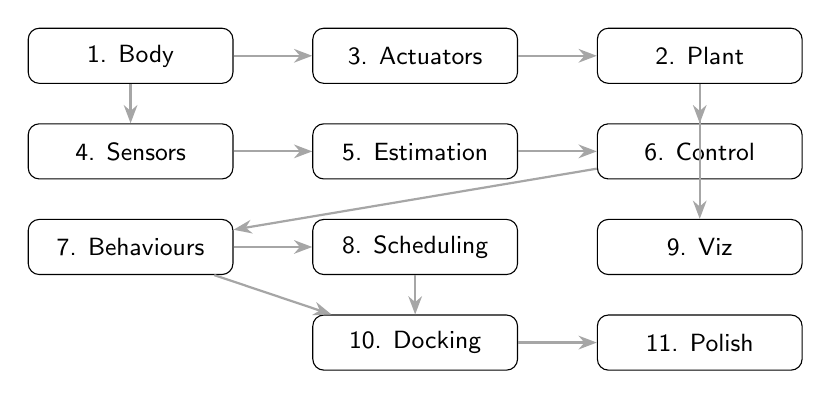
\begin{tikzpicture}[
    node distance=0.5cm and 1.0cm,
    n/.style={rectangle, draw, rounded corners, minimum height=0.7cm, minimum width=2.6cm, font=\small\sffamily, align=center},
    arr/.style={-{Stealth}, thick, gray!70},
]
    \node[n] (p1) {1. Body};
    \node[n, right=of p1] (p3) {3. Actuators};
    \node[n, right=of p3] (p2) {2. Plant};

    \node[n, below=of p1] (p4) {4. Sensors};
    \node[n, below=of p3] (p5) {5. Estimation};
    \node[n, below=of p2] (p6) {6. Control};

    \node[n, below=of p4] (p7) {7. Behaviours};
    \node[n, below=of p5] (p8) {8. Scheduling};
    \node[n, below=of p6] (p9) {9. Viz};

    \node[n, below=of p8] (p10) {10. Docking};
    \node[n, right=of p10] (p11) {11. Polish};

    \draw[arr] (p1) -- (p3);
    \draw[arr] (p3) -- (p2);
    \draw[arr] (p1) -- (p4);
    \draw[arr] (p4) -- (p5);
    \draw[arr] (p5) -- (p6);
    \draw[arr] (p2) -- (p6);
    \draw[arr] (p6) -- (p7);
    \draw[arr] (p7) -- (p8);
    \draw[arr] (p2) -- (p9);
    \draw[arr] (p7) -- (p10);
    \draw[arr] (p8) -- (p10);
    \draw[arr] (p10) -- (p11);
\end{tikzpicture}
\end{center}

\section{Validation checklist}

A single-page reference for end-of-phase sign-off. Tick when each test
passes:

\begin{itemize}[leftmargin=2em]
    \item[$\square$] Free body drifts at constant velocity (Phase~1).
    \item[$\square$] Constant force produces correct linear acceleration (Phase~1).
    \item[$\square$] Constant torque produces correct angular acceleration (Phase~1).
    \item[$\square$] Heading wraps correctly under sustained rotation (Phase~1).
    \item[$\square$] Forward / strafe / spin / diagonal scenarios produce expected trajectories (Phase~2).
    \item[$\square$] Ideal actuator stages without integrating (Phase~3).
    \item[$\square$] DC motor step response matches first-order model (Phase~3).
    \item[$\square$] Sensor noise statistics match configured values (Phase~4).
    \item[$\square$] Sensor refresh rates fire correctly (Phase~4).
    \item[$\square$] Passthrough estimator reproduces truth pose (Phase~5).
    \item[$\square$] Dead-reckoner drifts unboundedly without correction (Phase~5).
    \item[$\square$] EKF converges from wrong initialisation (Phase~5).
    \item[$\square$] EKF NIS is consistent (Phase~5).
    \item[$\square$] Robot reaches a single waypoint (Phase~6).
    \item[$\square$] Robot traces a square loop (Phase~6).
    \item[$\square$] Mode supervisor switches Cruise $\leftrightarrow$ Idle (Phase~7).
    \item[$\square$] Sensors and controllers honour their refresh rates (Phase~8).
    \item[$\square$] Live and batch visualisation both work (Phase~9).
    \item[$\square$] Nominal docking succeeds (Phase~10).
    \item[$\square$] Docking succeeds under dropout / latency / bias (Phase~10).
    \item[$\square$] \code{pip install -e .} works in a fresh venv (Phase~11).
    \item[$\square$] A second platform type compiles without changes to \code{sim2d.core} (Phase~11).
\end{itemize}

\end{document}
